% This must be in the first 5 lines to tell arXiv to use pdfLaTeX, which is strongly recommended.
\pdfoutput=1
% In particular, the hyperref package requires pdfLaTeX in order to break URLs across lines.

\documentclass[11pt]{article}

% Remove the "review" option to generate the final version.
%\usepackage[review]{acl}
\usepackage{acl}

% Standard package includes
\usepackage{times}
\usepackage{latexsym}

% For proper rendering and hyphenation of words containing Latin characters (including in bib files)
\usepackage[T1]{fontenc}
% For Vietnamese characters
% \usepackage[T5]{fontenc}
% See https://www.latex-project.org/help/documentation/encguide.pdf for other character sets

% This assumes your files are encoded as UTF8
\usepackage[utf8]{inputenc}

\usepackage{graphicx}
\usepackage{amsfonts}
\usepackage{amsmath}
\usepackage{amssymb}
\usepackage{bbm}
\usepackage{backnaur}



% This is not strictly necessary, and may be commented out,
% but it will improve the layout of the manuscript,
% and will typically save some space.
\usepackage{microtype}

\renewcommand{\bnfpn}[1]{\mathsf{#1}}
\renewcommand{\bnfpo}{\rightarrow}

% If the title and author information does not fit in the area allocated, uncomment the following
%
%\setlength\titlebox{<dim>}
%
% and set <dim> to something 5cm or larger.

\title{Towards More Natural Artificial Languages}

% Author information can be set in various styles:
% For several authors from the same institution:
% \author{Author 1 \and ... \and Author n \\
%         Address line \\ ... \\ Address line}
% if the names do not fit well on one line use
%         Author 1 \\ {\bf Author 2} \\ ... \\ {\bf Author n} \\
% For authors from different institutions:
% \author{Author 1 \\ Address line \\  ... \\ Address line
%         \And  ... \And
%         Author n \\ Address line \\ ... \\ Address line}
% To start a separate ``row'' of authors use \AND, as in
% \author{Author 1 \\ Address line \\  ... \\ Address line
%         \AND
%         Author 2 \\ Address line \\ ... \\ Address line \And
%         Author 3 \\ Address line \\ ... \\ Address line}

\author{Mark Hopkins \\
  Reed College \\
  \texttt{hopkinsm@reed.edu} \\}

\begin{document}
\maketitle
\begin{abstract}
tbd
\end{abstract}

\section{Introduction}

\section{Context-Free Grammars}

A context-free grammar (CFG) is a tuple $(N,\Sigma,S,R)$ where $N$ and $\Sigma$ are disjoint alphabets of symbols respectively called \emph{nonterminals} and \emph{terminals}, $S \in N$ is a distinguished nonterminal called the \emph{start symbol}, and $R$ is a set of strings called \emph{rules}. Each rule $r \in R$ has the form $A \bnfpo \beta$, where $A \in N$ and $\beta \in (N \cup \Sigma)^*$. The language $\mathcal{L}(G) \subseteq \Sigma^*$ defined by a CFG $G$ is the set of terminal sequences that can be produced by taking the start symbol $S$, and repeatedly substituting the left-hand symbol of a rule with its right-hand symbol string -- a process called a \emph{derivation}.

Figure~\ref{fig:pcfg1} shows a CFG\footnote{The vertical bar used in Figure~\ref{fig:pcfg1} is a shorthand for expressing multiple rules with a common left-hand side, e.g., $A \bnfpo \beta_1 \bnfor \beta_2$ represents the two rules $A \bnfpo \beta_1$ and $A \bnfpo \beta_2$.} that generates some simple English sentences like $\bnfts{it} \bnfsp \bnfts{drinks} \bnfsp \bnfts{water}$. Unfortunately, it also produces terminal sequences that are not grammatical English, like $\bnfts{you} \bnfsp \bnfts{drinks} \bnfsp \bnfts{water}$. To resolve this issue, we can refine the nonterminals to capture second and third person verb forms, as done in the grammar of Figure~\ref{fig:pcfg2}.


Among grammatical sentences, some are more common than others. A popular model of sentence likelihood is the probabilistic context-free grammar (PCFG). A PCFG augments a CFG with a function $q: R \rightarrow [0,1]$, which assigns a weight $q(r)$ to each rule $r \in R$ such that for each nonterminal $A \in N$:
\begin{equation*}
	\sum\limits_{\beta: A \bnfpo \beta \in R} q(A \bnfpo \beta) = 1
\end{equation*}
\noindent i.e. the weights of the rules with a common left-hand side sum to one. This induces a probability for each derivation: the product of the weights of the rules used in the derivation. More formal details can be found in REF. 

\begin{figure}
\begin{bnf*}
\bnfprod{S} {\bnfpn{NN} \bnfsp \bnfpn{VP}} \\
\bnfprod{VP} {\bnfpn{VB} \bnfsp \bnfpn{NN}}\\
\bnfprod{VB} {\bnfts{drink} \bnfor \bnfts{drinks} \bnfor \bnfts{eat} \bnfor \bnfts{eats}}\\
\bnfprod{NN} {\bnfts{you} \bnfor \bnfts{it} \bnfor \bnfts{water} \bnfor \bnfts{food}}
\end{bnf*}
\caption{A CFG describing a small subset of English.\label{fig:pcfg1}}
\end{figure}

\begin{figure}
\begin{bnf*}
\bnfprod{S} {\bnfpn{NN.2} \bnfsp \bnfpn{VP.2}} \\
\bnfprod{S} {\bnfpn{NN.3} \bnfsp \bnfpn{VP.3}} \\
\bnfprod{VP.2} {\bnfpn{VB.2} \bnfsp \bnfpn{NN}}\\
\bnfprod{VP.3} {\bnfpn{VB.3} \bnfsp \bnfpn{NN}}\\
\bnfprod{VB.2} {\bnfts{drink} \bnfor \bnfts{eat}}\\
\bnfprod{VB.3} {\bnfts{drinks} \bnfor \bnfts{eats}}\\
\bnfprod{NN} {\bnfpn{NN.2} \bnfor \bnfpn{NN.3}}\\
\bnfprod{NN.2} {\bnfts{you}}\\
\bnfprod{NN.3} {\bnfts{it} \bnfor \bnfts{water} \bnfor \bnfts{food}}
\end{bnf*}
\caption{A refinement of the CFG from Figure~\ref{fig:pcfg1} to eliminate ungrammatical sentences from the language.\label{fig:pcfg2}}
\end{figure}


\section{Modeling Selectional Preference}

Certain nouns appear more frequently as the object of a given verb. For instance, one is more likely to encounter a sentence like $\bnfts{it} \bnfsp \bnfts{drinks} \bnfsp \bnfts{water}$ than $\bnfts{it} \bnfsp \bnfts{drinks} \bnfsp \bnfts{food}$. This phenomenon, known as \emph{selectional preference}, cannot be modeled just by placing weights on the rules in Figure~\ref{fig:pcfg2}, since the weights associated with $\bnfpn{NN.3} \bnfpo \bnfts{water}$ and $\bnfpn{NN.3} \bnfpo \bnfts{food}$ are independent of the choice of verb.

\begin{figure}
\begin{bnf*}
\bnfprod{S} {\bnfpn{NN.2} \bnfsp \bnfpn{VP.2}} \\
\bnfprod{S} {\bnfpn{NN.3} \bnfsp \bnfpn{VP.3}} \\
\bnfprod{VP.2} {\bnfpn{VB.2.1} \bnfsp \bnfpn{NN.1}}\\
\bnfprod{VP.2} {\bnfpn{VB.2.2} \bnfsp \bnfpn{NN.2}}\\
\bnfprod{VP.3} {\bnfpn{VB.3.1} \bnfsp \bnfpn{NN.1}}\\
\bnfprod{VP.3} {\bnfpn{VB.3.2} \bnfsp \bnfpn{NN.2}}\\
\bnfprod{VB.2.1} {\bnfts{drink}} \\
\bnfprod{VB.3.1} {\bnfts{drinks}} \\
\bnfprod{VB.2.2} {\bnfts{eat}} \\
\bnfprod{VB.3.2} {\bnfts{eats}} \\
\bnfprod{NN.1} {\bnfpn{NN.2.1} \bnfor \bnfpn{NN.3.1}}\\
\bnfprod{NN.2} {\bnfpn{NN.2.2} \bnfor \bnfpn{NN.3.2}}\\
\bnfprod{NN.2.1} {\bnfts{you}}\\
\bnfprod{NN.2.2} {\bnfts{you}}\\
\bnfprod{NN.3.1} {\bnfts{it} \bnfor \bnfts{water} \bnfor \bnfts{food}}\\
\bnfprod{NN.3.2} {\bnfts{it} \bnfor \bnfts{water} \bnfor \bnfts{food}}
\end{bnf*}
\caption{A further refinement of the CFG from Figure~\ref{fig:pcfg2} to model selectional preference.\label{fig:pcfg3}}
\end{figure}

To create a PCFG that models selectional preference, we can further refine the nonterminals to encode the choice of verb. In Figure~\ref{fig:pcfg3}, we present a CFG with distinct rules $\bnfpn{VP.3} \bnfpo \bnfpn{VB.3.1} \bnfsp \bnfpn{NN.1}$ (for producing sentences whose verb is $\bnfts{drink}$) and $\bnfpn{VP.3} \bnfpo \bnfpn{VB.3.2} \bnfsp \bnfpn{NN.2}$ (for producing sentences whose verb is $\bnfts{eat}$). Through this refinement, the grammar produces the object from a nonterminal that encodes the verb, like $\bnfpn{NN.3.1}$ or $\bnfpn{NN.3.2}$, enabling us to assign verb-dependent probabilities to the terminal rules. For instance, we could assign a high probability to the rule $\bnfpn{NN.3.1} \bnfpo \bnfts{water}$ (because it common to drink water) and a low probability to the rule $\bnfpn{NN.3.1} \bnfpo \bnfts{food}$ (because it is uncommon to drink food).

Unfortunately, the prospect of engineering such a grammar (in particular, assigning the probabilities) is daunting, as languages contain a large number of verbs and nouns. Moreover, selectional preference occurs not only in verb-object relationships, but also verb-subject, noun-adjective, and verb-preposition relationships, among others. In this section, we introduce a framework for facilitating the creation of grammars that model selectional preference.

\subsection{Compound Symbols}

Define a \emph{signature} to be a tuple $\mathcal{S} = (N, \Sigma, Y, Z)$ of four pairwise disjoint alphabets, the symbols of which are respectively referred to as \emph{nonterminals}, \emph{terminals}, \emph{y-variables}, and \emph{z-variables}. As a notational convention, we will reserve symbols of the form $y_i$ and $z_i$ to represent elements of $Y$ and $Z$, respectively.

Given signature $\mathcal{S}$, define the set $C(\mathcal{S}) = (N \cup \Sigma \cup Y \cup Z \cup \mathbb{Z})^+$ of \emph{compound symbols}. A compound symbol will be written with periods separating its elements, e.g. if $\mathsf{VP} \in N$ and $y_4 \in Y$, then $\mathsf{VP}.y_4.7 \in C(\mathcal{S})$. It will be helpful to define the following subsets of $C(\mathcal{S})$:
\begin{itemize}
	\item $C_{\mathsf{left}}(\mathcal{S}) = (N \cup Y \cup \mathbb{Z})^+$
	\item $C_{\mathsf{right}}(\mathcal{S}) = (N \cup Y \cup Z)^+ \cup (\Sigma \cup Y \cup Z)^+$
	\item $C_{\mathsf{nt}}(\mathcal{S}) = (N \cup \mathbb{Z})^+$
	\item $C_{\mathsf{term}}(\mathcal{S}) = (\Sigma \cup \mathbb{Z})^+$
	\item $C_{\mathsf{wt}}(\mathcal{S}) = (Y \cup \mathbb{Z})^+$
	\item $C_{\mathsf{int}}(\mathcal{S}) = \mathbb{Z}^+$
\end{itemize}

A \emph{substitution} is a function $\sigma: D \rightarrow \mathbb{Z}$ with domain $D \subseteq Y \cup Z$. We extend the domain of a substitution to include any symbol that can appear in a compound symbol by defining:
\begin{gather*}
\bar{\sigma}(x) = \begin{cases}
         \sigma(x) &\mbox{ if } x \in D\\
         x &\mbox{ if } x \not\in D
       \end{cases}
\end{gather*}
\noindent for $x \in N \cup \Sigma \cup Y \cup Z \cup \mathbb{Z}$.

We apply a substitution $\sigma$ to a compound symbol $x_1.\cdots.x_n$ using the following definition:
\begin{equation*}
\sigma(x_1.\cdots.x_n) = \bar{\sigma}(x_1).\cdots.\bar{\sigma}(x_n)
\end{equation*}

\textbf{Example: } If substitution $\sigma = \{ y_1 \mapsto 52, z_1 \mapsto 14 \}$, then $\sigma(\mathsf{NN}.y_1.z_1) = \mathsf{NN}.52.14$.


\subsection{Grammar Macros}

A \emph{rule macro}\footnote{TODO: must also specify that the y-vars on the RHS must appear on the LHS.} with signature $\mathcal{S} = (N, \Sigma, Y, Z)$ is a string of the form $c \bnfpo \gamma$, where $c \in C_{\mathsf{left}}(\mathcal{S})$ and $\gamma \in (C_{\mathsf{right}}(\mathcal{S}))^*$. Define $V(\rho) \subseteq Y \cup Z$ as the set of variables that appear in at least one compound nonterminal of rule macro $\rho$. Similarly, we refer to the z-variables that appear in rule macro $\rho$ by defining $Z(\rho) = V(\rho) \cap Z$.

\textbf{Example: } For the following rule macro $\rho$, $V(\rho) = \{y_1, z_1\}$ and $Z(\rho) = \{z_1\}$:
\begin{equation*}
	\mathsf{VP}.y_1 \bnfpo \mathsf{VB}.y_1.z_1 \bnfsp \mathsf{NN}.z_1
\end{equation*}

\noindent Observe that z-variables can only appear on the right side of a rule macro, while y-variables can appear on either side.

We apply a substitution $\sigma$ to a rule macro $c \bnfpo \gamma_1.\cdots.\gamma_n$ as follows:
\begin{multline*}
\sigma(c \bnfpo \gamma_1.\cdots.\gamma_n) \\
= \sigma(c) \bnfpo \sigma(\gamma_1).\cdots.\sigma(\gamma_n)
\end{multline*}

\textbf{Example: } If substitution $\sigma = \{ y_1 \mapsto 3, z_1 \mapsto 14 \}$ and $\rho$ is the rule macro from the previous example, then $\sigma(\rho) =$
\begin{equation*}
	\mathsf{VP}.3 \bnfpo \mathsf{VB}.3.14 \bnfsp \mathsf{NN}.14
\end{equation*}

A \emph{grammar macro} is a tuple $(\mathcal{S}, S, \mathcal{R})$ where $\mathcal{R}$ is a set of rule macros with signature $\mathcal{S}$ and $S \in C_{\mathsf{nt}}(\mathcal{S})$ is a distinguished symbol called the \emph{start symbol}. Figure~\ref{fig:gmacro1} shows an example grammar macro.

\begin{figure}
\begin{bnf*}
\bnfprod{S} {\bnfpn{NN.z_1} \bnfsp \bnfpn{VP.z_1}} \\
\bnfprod{VP.y_1} {\bnfpn{VB.y_1.z_1} \bnfsp \bnfpn{NN.z_1}}\\
\bnfprod{VB.y_1.y_2} {\bnfts{verb}.\bnfpn{y_1.y_2}} \\
\bnfprod{NN.y_1} {\bnfpn{NN.y_1.z_1}} \\
\bnfprod{NN.y_1.y_2} {\bnfts{noun}.\bnfpn{y_1.y_2}}
\end{bnf*}
\caption{An example grammar macro that can produce simple subject-verb-object sentences.\label{fig:gmacro1}}
\end{figure}


As the name implies, a grammar macro is a compact way of describing a grammar. Each rule macro $\rho$ induces a set of rules:
\begin{equation*}
	R(\rho) = \{\sigma(\rho) \mid \sigma: V(\rho) \rightarrow \mathbb{Z} \}
\end{equation*}

A grammar macro $M = (\mathcal{S}, S, \mathcal{R})$ 
induces a CFG containing the union of these rules:
\begin{equation*}
G(M) = (C_{\mathsf{nt}}(\mathcal{S}),C_{\mathsf{term}}(\mathcal{S}),S, \bigcup_{\rho \in \mathcal{R}} R(\rho))
\end{equation*}

The example grammar macro in Figure~\ref{fig:gmacro1} induces a CFG that is similar to the CFG from Figure~\ref{fig:pcfg3}. There are two differences. First, the induced CFG contains \emph{all} rules of the form $\bnfpn{S} \bnfpo \bnfpn{NN.z_1} \bnfsp \bnfpn{VP.z_1}$, not just $\bnfpn{S} \bnfpo \bnfpn{NN.2} \bnfsp \bnfpn{VP.2}$ and $\bnfpn{S} \bnfpo \bnfpn{NN.3} \bnfsp \bnfpn{VP.3}$. In the next section, we will show how to augment the macro with probabilities so that we can effectively eliminate undesired rules like $\bnfpn{S} \bnfpo \bnfpn{NN.4} \bnfsp \bnfpn{VP.4}$.

The second difference is that the terminal rules generate generic words like $\bnfts{verb.3.1}$ and $\bnfts{verb.3.2}$ (the 3rd person form of verbs 1 and 2 in our language) rather than the actual lexical forms $\bnfts{drink}$ and $\bnfts{eat}$. This difference can be resolved by pairing the grammar macro with a \emph{voicebox}, defined as a function $\beta: C_{\mathsf{term}}(\mathcal{S}) \mapsto V$ that maps the compound terminals to words of a vocabulary $V$. Tokens of the language $\mathcal{L}(G(M))$ can be postprocessed by the voicebox to create the desired lexemes.

\subsection{Weighted Grammar Macros}

Finally, we show how to extend grammar macros to induce WCFGs. Define an \emph{integer weighting} as a function $\mathbb{Z} \mapsto [0,\infty)$ that assigns a nonnegative weight to each integer. Observe that any probability distribution over integers is an integer weighting (and all of our examples will be probability distributions). When we provide example integer weightings, any unspecified integer will be assumed by convention to map to zero, e.g. if we specify integer weighting $w_\mathsf{int} = \{3 \mapsto 0.3, 5 \mapsto 0.7\}$, then $w_\mathsf{int}(4) = 0$.

Define a \emph{weighting table} as a function $\tau$ that assigns integer weightings to a subset of the compound symbols in set $C_{\mathsf{int}}(\mathcal{S})$. Define a \emph{z-weighting} of rule macro $\rho$ as a function $\zeta: Z(\rho) \rightarrow C_{\mathsf{wt}}(\mathcal{S})$ that assigns a compound symbol to each z-variable of the rule macro.

A \emph{weighted grammar macro} is a tuple $(M, w_\theta, w_\zeta, \tau)$ where:
\begin{itemize}
	\item $M = (\mathcal{S}, S, \mathcal{R})$ is a grammar macro
	\item $w_\theta: \mathcal{R} \rightarrow [0,\infty)$ is a function that assigns a nonnegative weight (called the \emph{base weight} to each rule macro $\rho \in \mathcal{R}$
	\item $w_\zeta$ is a function that assigns a z-weighting to each rule macro $\rho \in \mathcal{R}$
	\item $\tau$ is a weighting table
\end{itemize}

\noindent A weighted grammar macro induces a WCFG $(G(M), q)$ where $q$ assigns the following weight to each rule $r = \sigma(\rho)$ of CFG $G(M)$ induced from rule macro $\rho$ via substitution $\sigma$:
\begin{equation*}
	q(r) = w_\theta(\rho) \cdot \prod\limits_{z \in Z(\rho)} w_\mathsf{int}(\sigma(z))
\end{equation*}
\noindent where $w_\mathsf{int} = \tau(\sigma(w_\zeta(\rho)))$ is the integer weighting assigned to compound symbol $\sigma(w_\zeta(\rho))$ in the weighting table $\tau$.

\begin{figure}
\begin{tabular}{rcl|l|l} 
&&&$w_\theta$&$w_\zeta$\\
\hline \hline
$\bnfpn{S}$ &$\bnfpo$& $\bnfpn{NP.z_1}$ & 1.0 & $\bnfpn{z_1} \mapsto \bnfpn{1}$ \\
$\bnfpn{NP.y_1}$ &$\bnfpo$& $\bnfpn{ADJ.z_1} \bnfsp \bnfpn{NN.y_1}$ & 1.0 & $\bnfpn{z_1} \mapsto \bnfpn{2.y_1}$\\
$\bnfpn{ADJ.y_1}$ &$\bnfpo$& $\bnfts{adj}.\bnfpn{y_1}$ & 1.0 &\\
$\bnfpn{NN.y_1}$ &$\bnfpo$& $\bnfts{noun}.\bnfpn{y_1}$ & 1.0 &
\end{tabular}
\caption{An example weighted grammar macro that produces simple noun phrases.\label{fig:gmacro2}}
\end{figure}


\textbf{Example: } Figure~\ref{fig:gmacro2} partially specifies a weighted grammar macro (the weighting table is left unspecified) that generates simple phrases consisting of a single adjective and noun. Suppose that the weighting table contains the mapping $\tau(\bnfpn{2.3}) = \{4 \mapsto 0.3, 5 \mapsto 0.7\}$. Then the induced rule $\bnfpn{NP.3} \bnfpo \bnfpn{ADJ.4} \bnfsp \bnfpn{NN.3}$ has weight $0.3$, the induced rule $\bnfpn{NP.3} \bnfpo \bnfpn{ADJ.5} \bnfsp \bnfpn{NN.3}$ has weight $0.7$, and the induced rule $\bnfpn{NP.3} \bnfpo \bnfpn{ADJ.6} \bnfsp \bnfpn{NN.3}$ has weight 0.

Figure~\ref{fig:gmacro2} is an example of a head-driven grammar macro, in which we first determine the head word (in this case, the noun) by drawing it from a general noun distribution $\tau(1)$, then we produce the dependent (in this case, a modifying adjective) from a distribution $\tau(\bnfpn{2.y_1})$ that depends on the selected head $\bnfts{noun}.\bnfpn{y_1}$. This enables us to model selectional preference between head words and their dependents.


\section{Modeling the Power Law Distributions of Natural Language}


We now turn our attention to devising weighted grammar macros that emulate natural language, using Figure~\ref{fig:gmacro2} as a case study. Our aim is to associate Figure~\ref{fig:gmacro2} with a weighting table $\tau$ such that the produced language emulates the statistics of natural language noun phrases. Specifically, we will attempt to identify appropriate probability distributions\footnote{Recall from the previous section that probability distributions are integer weightings whose range sums to one.} $\tau(\bnfpn{1})$ and $\tau(\bnfpn{2.y_1})$. 

\begin{figure}[t]
\centering
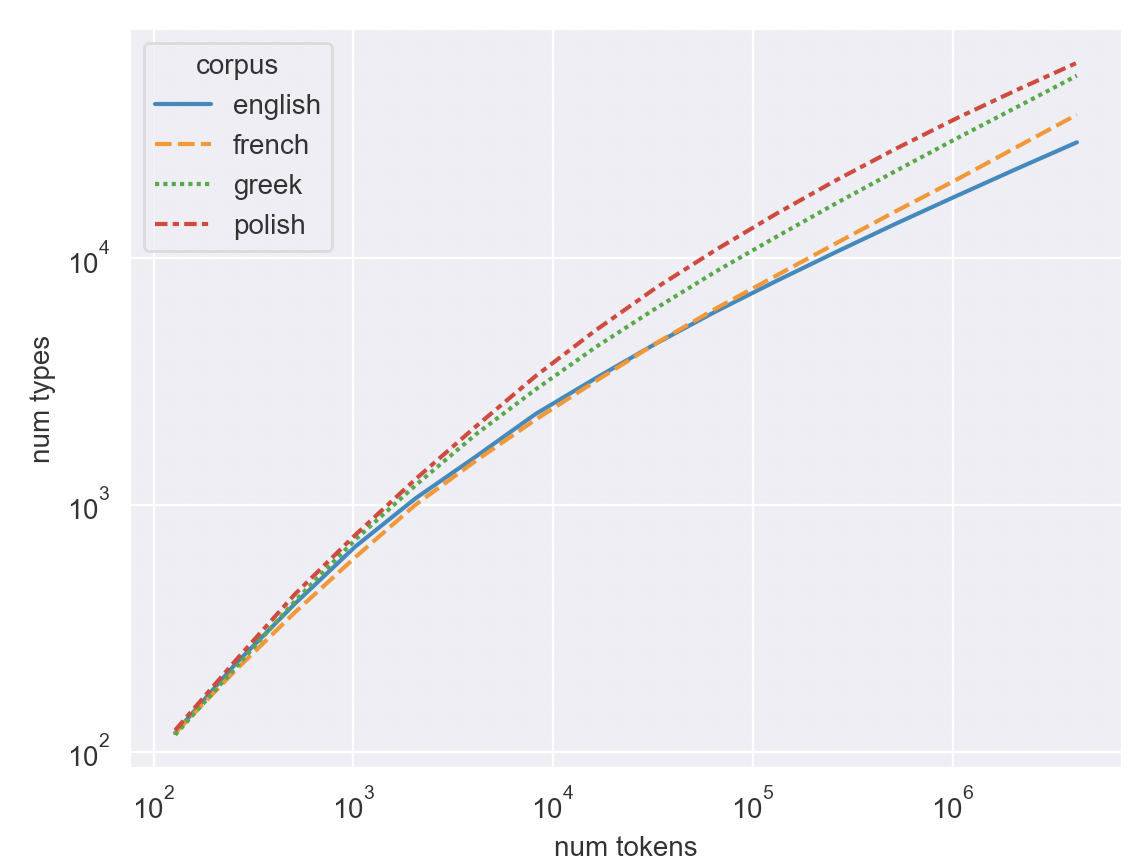
\includegraphics[width=0.48\textwidth]{images/type_token1.png}
\caption{Number of noun types versus number of observed noun tokens in the Europarl corpus.}
\label{fig:type_token1}
\end{figure}

\begin{figure}[t]
\centering
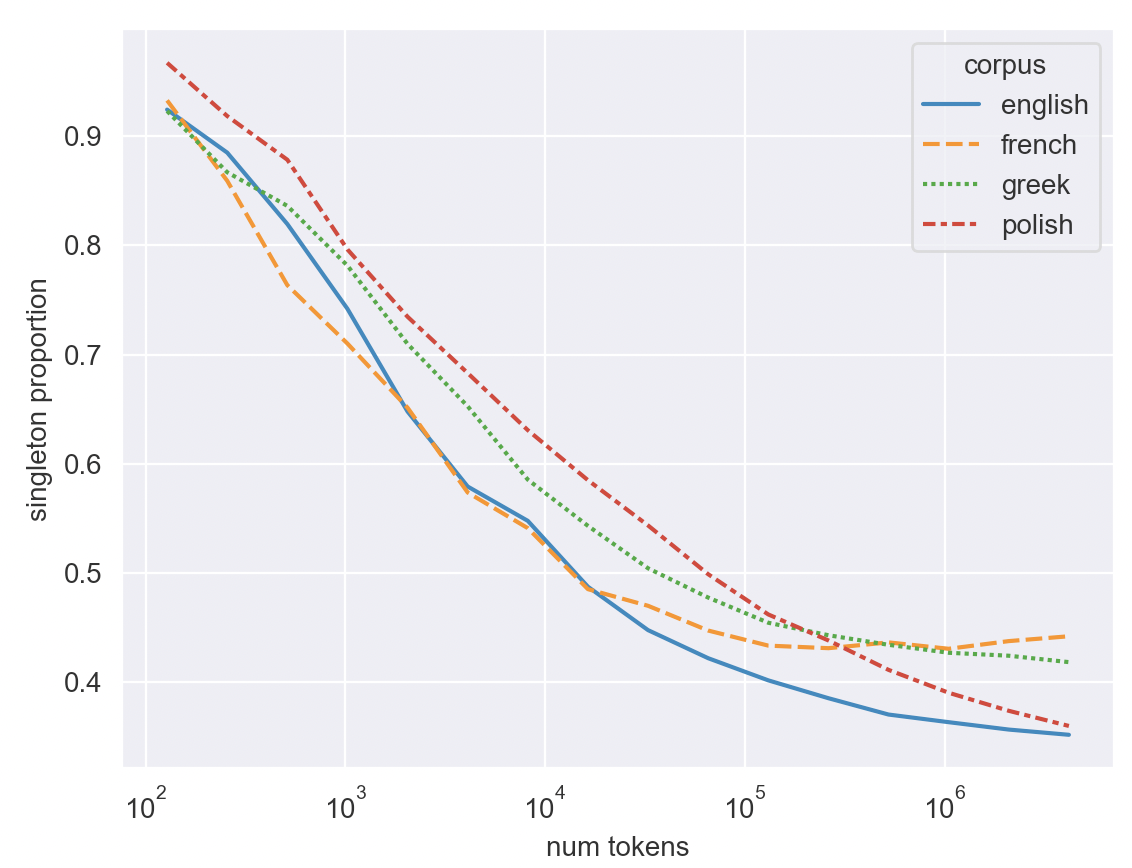
\includegraphics[width=0.48\textwidth]{images/sp1.png}
\caption{Singleton proportion versus number of observed noun tokens in the Europarl corpus.}
\label{fig:sp1}
\end{figure}

\subsection{Pitman-Yor Processes}

Let's begin by considering the noun distribution $\tau(\bnfpn{1})$. One strategy could be to collect a histogram of nouns from a corpus and normalize the histogram to create the distribution. But this commits us to a vocabulary size and token probabilities that are specific to the size of the corpus. This will be inappropriate for generating larger corpora, because nouns are an ``open class" of tokens whose frequencies follow a power law distribution. In Figure~\ref{fig:type_token1}, we plot the number of noun types (i.e. unique nouns) versus noun tokens for increasingly large subsets of the Europarl corpus (CITE). Observe that the number of types never converges -- new nouns continue to be discovered, no matter how large the corpus grows\footnote{The languages with richer morphology, Polish and Greek, have a higher type-token ratio than more analytic languages like English and French, but the ``heavy tail" phenomenon manifests regardless of the language's morphological properties.}. This ``heavy tail" property of natural language tokens has been documented by \cite{newman2005power} and \cite{teh-2006-hierarchical}, among others.

Another way to visualize this property \cite{teh-2006-hierarchical} is to plot the proportion of singleton tokens against the overall number of observed\footnote{To generate Figures~\ref{fig:type_token1} and \ref{fig:sp1}, we shuffled the Europarl sentences and extracted the nouns using \texttt{spaCy}. The shuffling smooths irregularities caused by topic shift.} tokens. Notice that the singleton proportion appears to converge to somewhere between 30\% and 50\% as the corpus size grows -- another indicator that in natural language, we continue to encounter new tokens, no matter how many tokens have already been observed.

To model this behavior, \cite{teh-2006-hierarchical} suggests using a generalization of the Dirichlet distribution \cite{kotz2004continuous} known as the Pitman-Yor process \cite{pitman1997two}. A Pitman-Yor process $\mathsf{PY}(d, \theta, G_0)$ is characterized by a \emph{discount} parameter $d \in [0,1)$, a \emph{strength} parameter $\theta \in (-d,\infty)$, and a \emph{base distribution} $G_0$ over integers $\{1, ..., V\}$. We follow \cite{teh-2006-hierarchical} in describing a Pitman-Yor process as a stochastic process that generates samples $\langle x_1, x_2, ... \rangle$ from i.i.d. samples $\langle y_1, y_2, ... \rangle$ drawn from base distribution $G_0$. Intuitively, it is a ``rich-get-richer" process, in which the $j$th sample $x_j$ is set to either a value $y_i$ assigned to a previous $x$-sample (with probability proportional to how many previous $x$-samples have been set to $y_i$), or the next $y$-sample in the sequence that hasn't yet been used. Formally, let $b_1=1$ and draw subsequent binary values $b_{n+1}$ from a Bernoulli (coin-flip) distribution where:
\begin{equation*}
	P(b_{n+1} = 1) =\frac{\theta + d\sum\limits_{1 \leq i \leq n} b_i}{\theta + n} 
\end{equation*}

\noindent Now define $t_1 = 1$ and consider $j, n \in \mathbb{Z}^+$. If $b_{n+1}=0$, then let $t_{n+1}=j$ with probability:
\begin{equation*}
	\frac{1}{n} \sum\limits_{1 \leq i \leq n} \mathbbm{1}(t_i=j)
\end{equation*}
Otherwise, if $b_{n+1}=1$: 
\begin{equation*}
t_{n+1}=1 + \sum\limits_{1 \leq i \leq n} b_i
\end{equation*}

\noindent The $n$th sample drawn from the Pitman-Yor process is $x_n = y_{t_n}$.

A Pitman-Yor process, for all practical purposes, can generate an "open-class" of words by using a uniform base distribution $G_0$ with a sufficiently large vocabulary size $V$ (for our experiments, we use the space of all 32-bit integers). However, we still need to choose appropriate discount and strength parameters.

\begin{figure}[t]
\centering
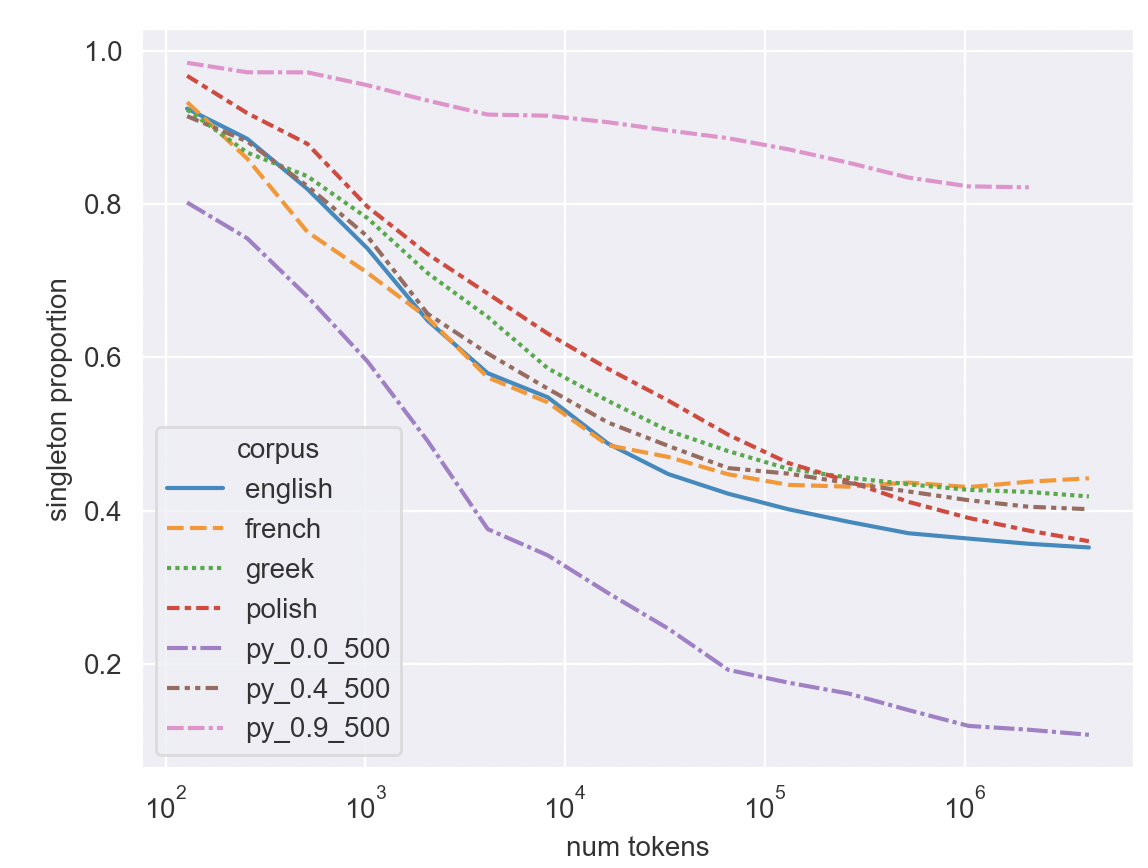
\includegraphics[width=0.48\textwidth]{images/sp2.png}
\caption{A comparison of the singleton proportion curves generated by Pitman-Yor processes with the curves of observed noun tokens in the Europarl corpus.}
\label{fig:sp2}
\end{figure}

\begin{figure}[t]
\centering
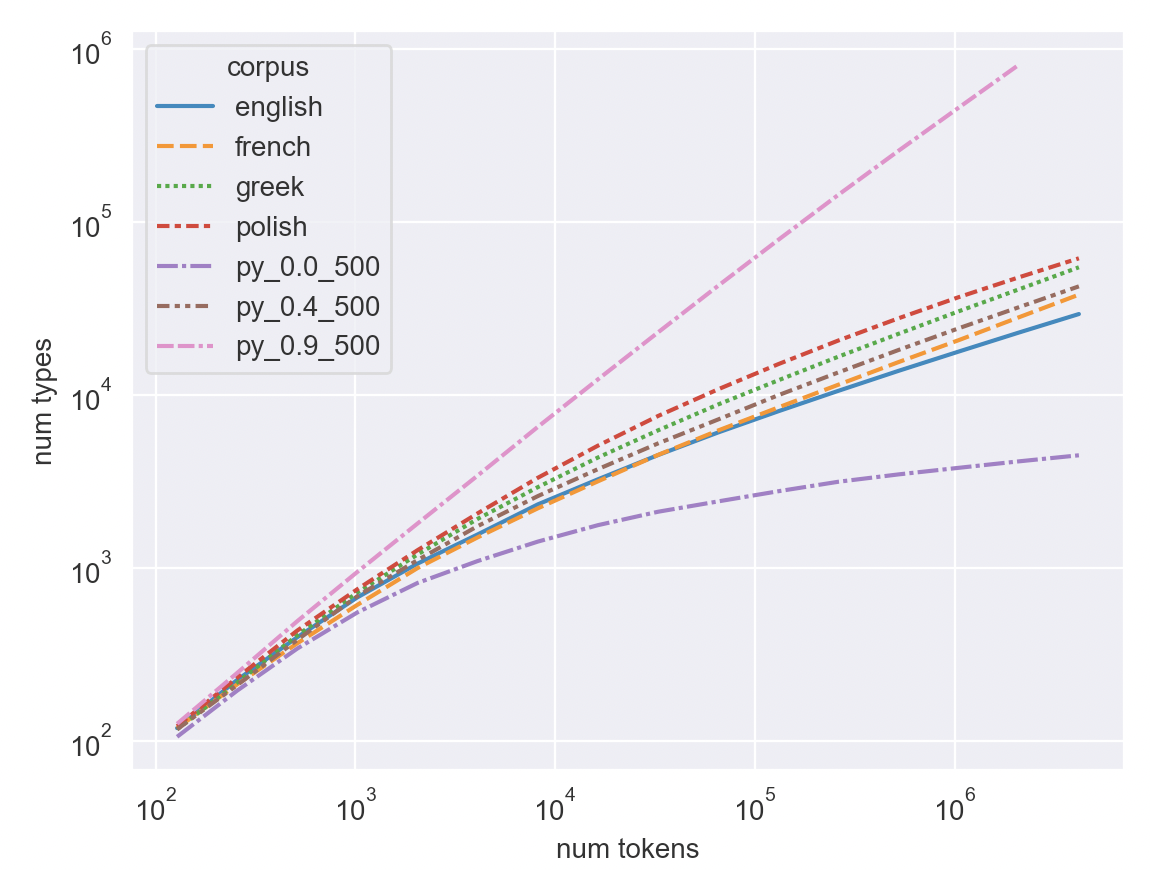
\includegraphics[width=0.48\textwidth]{images/type_token2.png}
\caption{A comparison of the type-token ratio curves generated by Pitman-Yor processes with the curves of observed noun tokens in the Europarl corpus.}
\label{fig:type_token2}
\end{figure}


In Figure~\ref{fig:sp2}, we plot the singleton proportion curves of tokens generated by various Pitman-Yor processes, and compare them with the singleton proportion curves of Europarl nouns. We find that $\mathsf{PY}(0.4, 500, G_0)$ closely follows the natural language curves. We obtain a similar correspondence when we plot the number of types versus the number of tokens (Figure~\ref{fig:type_token2}).


\subsection{Hierarchical Pitman-Yor Processes}

A similar experiment shows that $\mathsf{PY}(0.4, 500, G_0)$ also closely mirrors the natural language statistics of adjectives across the selected Europarl languages. So what happens if we use the distribution $\mathsf{PY}(0.4, 500, G_0)$ for both the noun distribution (i.e. distribution $\bnfpn{1}$) and every adjective distribution $\bnfpn{2.y_1}$) of the weighted grammar macro in Figure~\ref{fig:gmacro2}? In other words, what if we ignore selectional preference and just create adjective distributions that are independent of the head noun?

\begin{figure}[t]
\centering
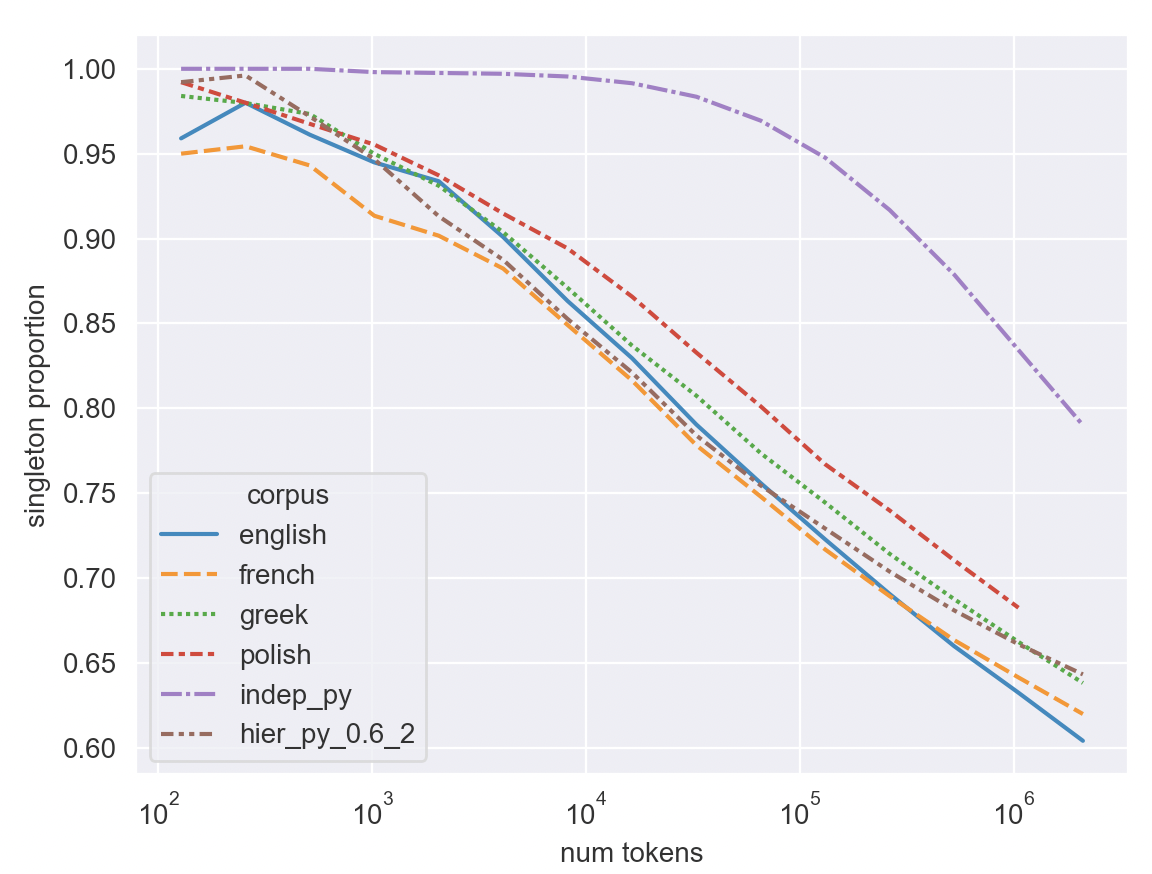
\includegraphics[width=0.48\textwidth]{images/sp3.png}
\caption{A comparison of the singleton proportion curves of adjective-noun bigrams in the Europarl corpus with bigrams generated from the macro in Figure~\ref{fig:gmacro2} using independent and hierarchical Pitman-Yor processes.}
\label{fig:sp3}
\end{figure}

\begin{figure}[t]
\centering
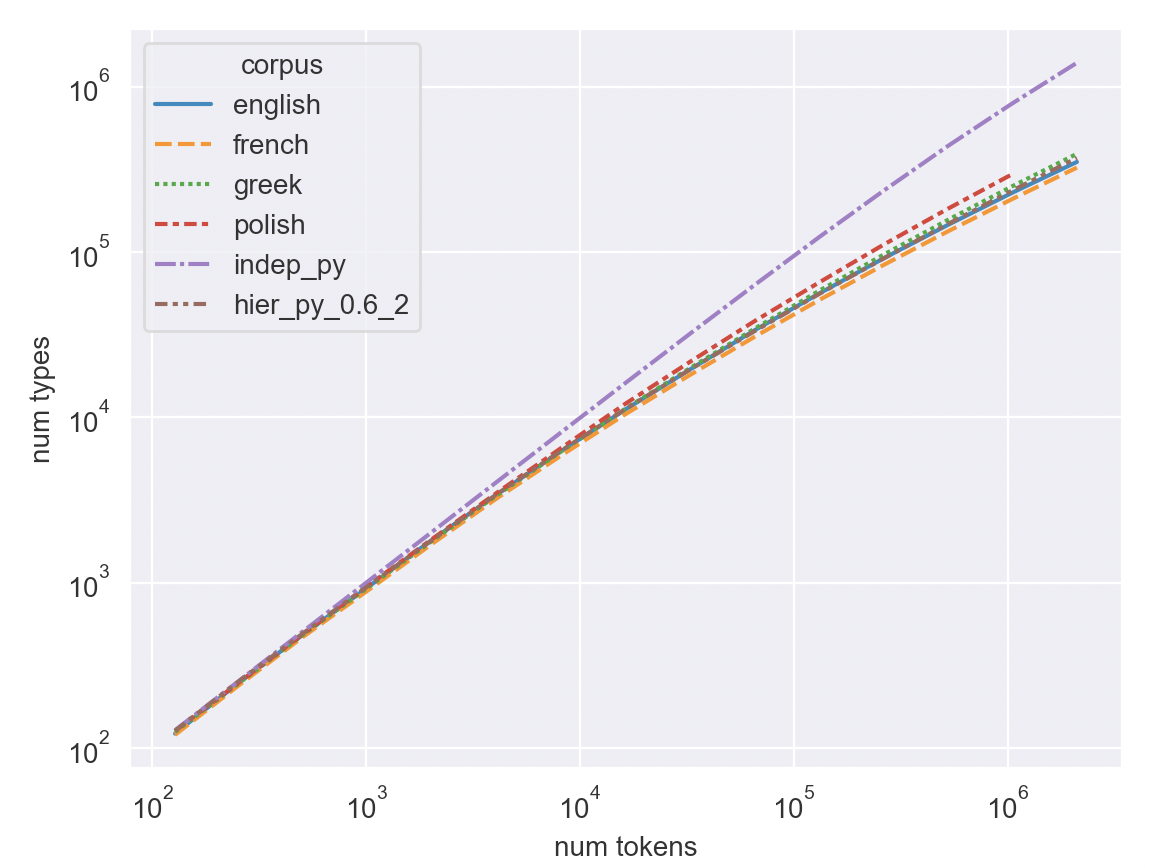
\includegraphics[width=0.48\textwidth]{images/type_token3.png}
\caption{A comparison of the type-token ratio curves of adjective-noun bigrams in the Europarl corpus with bigrams generated from the macro in Figure~\ref{fig:gmacro2} using independent and hierarchical Pitman-Yor processes.}
\label{fig:type_token3}
\end{figure}

To see what happens, we extract the adjective-noun bigrams from Europarl\footnote{We used spaCy to obtain universal dependency parses (CITE) of the sentences, then extracted adjective-noun pairs related by the $\texttt{amod}$ dependency.} and plot singleton proportion curves of these extracted bigrams in Figure~\ref{fig:sp3}. The adjective-noun bigrams generated from independent distributions bear little resemblance to the natural language curves, confirming the importance of generating the adjectives from a noun-dependent distribution. To do so, we make use of a \emph{hierarchical Pitman-Yor process} \cite{teh-2006-hierarchical}.

A hierarchical Pitman-Yor process is simply a Pitman-Yor process that uses another Pitman-Yor process as its base distribution. For instance, we can define a global adjective distribution $G_\mathsf{2} = \mathsf{PY}(0.4, 500, G_0)$, and then for each noun $\bnfts{noun}.\bnfpn{y_1}$, we define a noun-dependent adjective distribution $G_\mathsf{\bnfpn{2.y_1}} = \mathsf{PY}(d, \theta, G_\bnfpn{2})$. Figure~\ref{fig:sp3} shows that using discount $d=0.6$ and strength $\theta=2$ (with base distribution $\mathsf{PY}(0.4, 500, G_0)$) provides a close match to the singleton proportion curves of natural language. The type-token ratio curves (Figure~\ref{fig:type_token3}) tell the same story. 

\section{Experiments}

We repeat the methodology of \cite{white-etal-2021-non}


\bibliography{anthology,custom}
\bibliographystyle{acl_natbib}

\appendix

\end{document}
